\documentclass[10pt]{article}
\usepackage{ctex}
\usepackage{CJK}
\usepackage{graphicx}
\usepackage{graphicx}
\bibliographystyle{plain}
\setlength{\parindent}{2em}
\begin{document}
\title{Smart phone enterprise}
\author{Qilei Zhang}
\date{may 13 2018}
\maketitle
\par
\begin{figure}[htbp]
\small
\centering
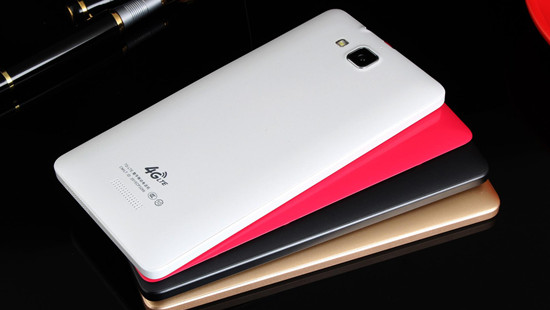
\includegraphics[width=20em]{smart.jpg}
\caption{Figure:Smart phone enterprise}
\label{fig:lable}
\end{figure}
\par
\section{background}
Chinese mainland companies took 10 spots among the world's top 14 smartphone suppliers in 2016, according to a recent report by market research institute IC Insights. The shipments of Chinese smartphone brands Huawei, OPPO, Vivo, ZTE, Lenovo, Xiaomi, TCL, Gionee, Meizu and LeEco/Coolpad totaled 587 million units last year, with a combined market share of 39 percent, according to the report.\cite{higham1994bibtex}
\par
\section{text}
With the rapid development of science and technology in China, the output of Chinese smart phone companies is increasing. China has a large population, a large demand for smart phones, and abundant labor resources in China, which is conducive to the production of large numbers of smart phones.\cite{h1994bibtex}
\par
With the rapid development of China's economy, more and more countries recognize Chinese products, and the quality of mobile phones is getting better and better. Apple and Samsung continued to dominate the smartphone market in 2016, but their combined shipment slipped from 555 million units in 2015 to 526 million in 2016, with market shares dropping four percentage points to 35 percent. Chinese smart phones have higher cost performance, so more and more people use domestic mobile phones.\\
\par
\begin{tabular}{|c|c|c|c|c|c|p{20em}}
\hline
company  & Samsung & Apple & Huawei&OPPO&xiaomi\\
\hline
ranking  &   1     &  2    &   3   & 4  &  5\\
\hline
\end{tabular}
\bibliography{aaa}
\footnote{\centering Smart phone enterprise}
\end{document}

